\documentclass[11pt]{article}

\usepackage[utf8]{inputenc}
\usepackage[T1]{fontenc}
\usepackage{mathptmx}
% \usepackage[skip=3em]{caption}

\topmargin -4em
\setlength{\textwidth} {420pt}
\setlength{\textheight} {620pt}
\setlength{\oddsidemargin} {20pt}
\setlength{\marginparwidth} {72in}


\usepackage{fancyhdr}
\usepackage{hyperref}
\usepackage{graphicx}
\usepackage{subcaption}
\usepackage{mathtools}

% may not work with travis ci
\usepackage{color}

% Use elastic spacing around the headers
\usepackage{titlesec}
\titlespacing\section{0pt}{6pt plus 4pt minus 2pt}{4pt plus 2pt minus 2pt}

% set it so that subsubsections have numbers and they
% are displayed in the TOC (maybe hard to read, might want to disable)
\setcounter{secnumdepth}{3}
\setcounter{tocdepth}{3}

% define widow protection
\def\widow#1{\vskip #1\vbadness10000\penalty-200\vskip-#1}

\clubpenalty=10000  % Don't allow orphans
\widowpenalty=10000 % Don't allow widows

% this should give you the ability to use some math symbols that
% were available by default in standard latex (i.e. \Box)
\usepackage{latexsym}

% define a little section heading that doesn't go with any number
\def\littlesection#1{
  \widow{2cm}
  \vskip 0.5cm
  \noindent{\bf #1}
  \vskip 0.0001cm
}

\pagestyle{fancyplain}

\newcommand{\tstamp}{\today}


% \renewcommand{\sectionmark}[1]{\markright{#1}}
% \lhead[\Section \thesection]            {\fancyplain{}{\rightmark}}
% \chead[\fancyplain{}{}]                 {\fancyplain{}{}}
% \rhead[\fancyplain{}{\rightmark}]       {\fancyplain{}{\thepage}}
% \cfoot[\fancyplain{\thepage}{}]         {\fancyplain{\thepage}{}}
%
% \newlength{\myVSpace}% the height of the box
% \setlength{\myVSpace}{1ex}% the default,
% \newcommand\xstrut{\raisebox{-.5\myVSpace}% symmetric behaviour,
%   {\rule{0pt}{\myVSpace}}%
% }

% leave things with no spacing extra spacing in the final version of the paper
\renewcommand{\baselinestretch}{1.0} % must go before the begin of doc

% suppress the use of indentation for a paragraph
\setlength{\parindent}{0.0in}
\setlength{\parskip}{0.1in}


% custom commands
\newcommand{\name}{{\sc RayTerm}}
\newcommand{\rayorg}{\vec{R_{origin}}}
\newcommand{\raydir}{\vec{R_{direction}}}

\newcommand\todo[1]{
\begin{center}
  \color{red}
  {\bf TODO}\\
  #1
\end{center}
}

% begin actual document

\begin{document}

% handle widows appropriately
\def\widow#1{\vskip #1\vbadness10000\penalty-200\vskip-#1}

% make the title section

\thispagestyle{empty}
\begin{center}
  {\Huge
    \name
    \par
  }
  {\LARGE
    A Ray-Tracing Rendering Engine for XTerm-like Terminals
    \par
  }
  {\normalsize
    Saejin Mahlau-Heinert \\
    Department of Computer Science \\
    Allegheny College \\
    {\tt mahlauheinerts@allegheny.edu} \\
    \url{https://saejinmh.com} \\
    \vspace*{.1in} \today \\ \vspace*{.1in}
    \par
  }
  \vskip 2em
\end{center}

% Default "abstract" environment is too small; customize one instead:
\begin{center}
  \large\bf Abstract
  \vspace{-1em}
\end{center}

\begin{quote}

Over the many years of innovation in the field of computer graphics, advances in rendering have led to massive increases in the fidelity of engaging, satisfying, and realistic computer visualizations.
\name\ is a new and unique entry into the ranks of rendering engines, and makes its own contributions to the field of computer graphics.
While harkening back to the retro aesthetics of the seventies and eighties, \name\ embraces new advances in computing power to bring fully ray-traced visuals to an old screen -- the terminal.
Using Unicode block characters to simulate pixels and a ray-tracer written in C++, a fully three dimensional scene will be rendered, complete with lighting, shadows, and physically-based materials.
\name\ can be used as an engine for terminal-based 3D tools, visualizations, games, and more; it will be fully open-source and ready for integration into other projects.

\end{quote}

\section{Introduction}
\label{sec:introduction}

% Provide an intuitive motivation for and introduction to your proposed senior thesis research.
% Whenever possible, you should use one or more concrete examples and technical diagrams.

In the early days of computing, real-time rendering engines that powered games like {\it Doom} or {\it NetHack} had to run on extremely underpowered hardware and render on low-resolution screens.
The dream of real-time, photorealistic graphics was far, far away.
However, even then the simple, blocky graphics, easily recognizable shapes, and maze-like environments were fantastic entertainment.
Today the retro-style of low-resolution graphics, pixel art, and 8-bit color is abound in the gaming space.
This proposal is one part of enabling that retro-aesthetic to grow into a new and unique style that, while similar to the old classics, can be more engaging and real than they ever were.
With the current generation of powerful CPU and GPU chips, able to execute billions and trillions of calculations per second respectively, it is finally possible to do real-time, close to photorealistic rendering.
While the goal of \name\ is not high-resolution photorealism, some approximation of photorealism will be obtained, albeit at a lower resolution.


This proposal describes \name, a system that will create what are, in essence, images on a terminal screen.
This rendering engine will perform real-time updating of the displayed image, generating an animation.
\name\ will use the recursive ray-tracing algorithm, simulating the path of light through the scene -- this is described in more detail in Section~\ref{sec:introduction:raytracing}.
Rendered images will be displayed in two different modes: using single half-character pixels, or more complex Unicode block characters.
The mechanics of this image composition method are discussed in Section~\ref{sec:introduction:unicode}.
Once an image is rendered, the \texttt{ncurses} C library \cite{ncursesLibrary} will be used to display it in a terminal.
The final terminal output will be similar to Figure~\ref{fig:checker_metal}, which was generated by TerminalImageViewer \cite{tivGithub} as a mockup.
More details on this process are given in Section~\ref{sec:introduction:ncurses}.


\begin{figure}[htb]
  \centering
  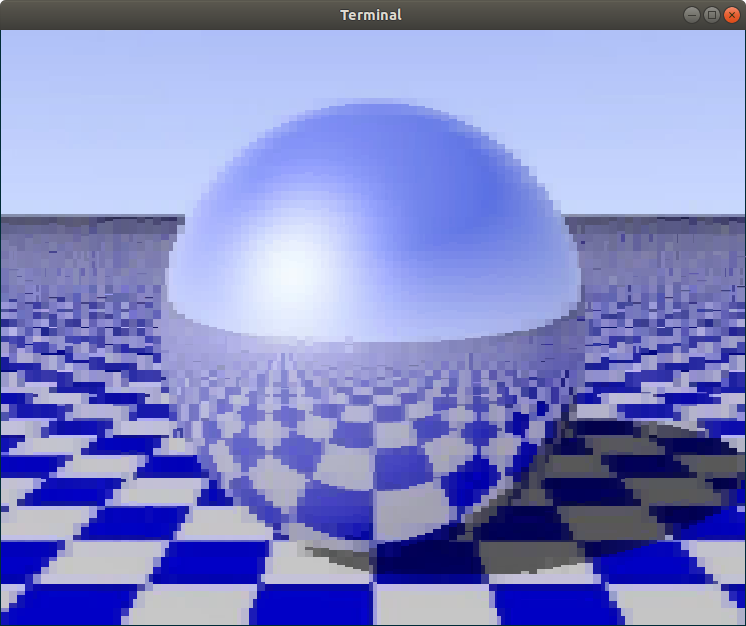
\includegraphics[width=0.8\textwidth]{resources/checker_metal}
  \caption{Example of proposed terminal output}
  \label{fig:checker_metal}
\end{figure}

\subsection{Rendering Engines and Ray-Tracing}
\label{sec:introduction:raytracing}

A rendering engine is an algorithm that takes a scene -- a description of some collection of objects -- and generates an image or visual representation of that scene.
There are many different algorithms that accomplish this goal.
In this proposal, the recursive ray-tracing algorithm first pioneered by Turner Whitted in his ground-breaking paper {\it An Improved Illumination Model for Shaded Display} \cite{whitted1980improved}, will be discussed and utilized.
Ray-tracing was one of the first algorithms developed in the field of computer graphics, and although there have been some improvements since then, the idea behind the algorithm has maintained its original simplicity.

Ray-tracing has been used as the renderer of choice for photorealistic images, because with only a few modifications to Whitted's original algorithm, it can generate fantastic images.
In the past, however, render times have been so slow that it was impossible to generate images fast enough for real-time use.
For example, Figure~\ref{fig:povray_render} is a render created by the POV-Ray engine \cite{povray}.
POV-Ray can take between a few minutes to several hours to complete one single image depending on the processing power involved.
However, there have been a few recent innovations that change this, such as NVIDIA's RTX hardware acceleration.
Section~\ref{sec:method} provides more details on these advances, as well as an explanation of how ray-tracing will be utilized in \name.

\begin{figure}[htb]
  \centering
  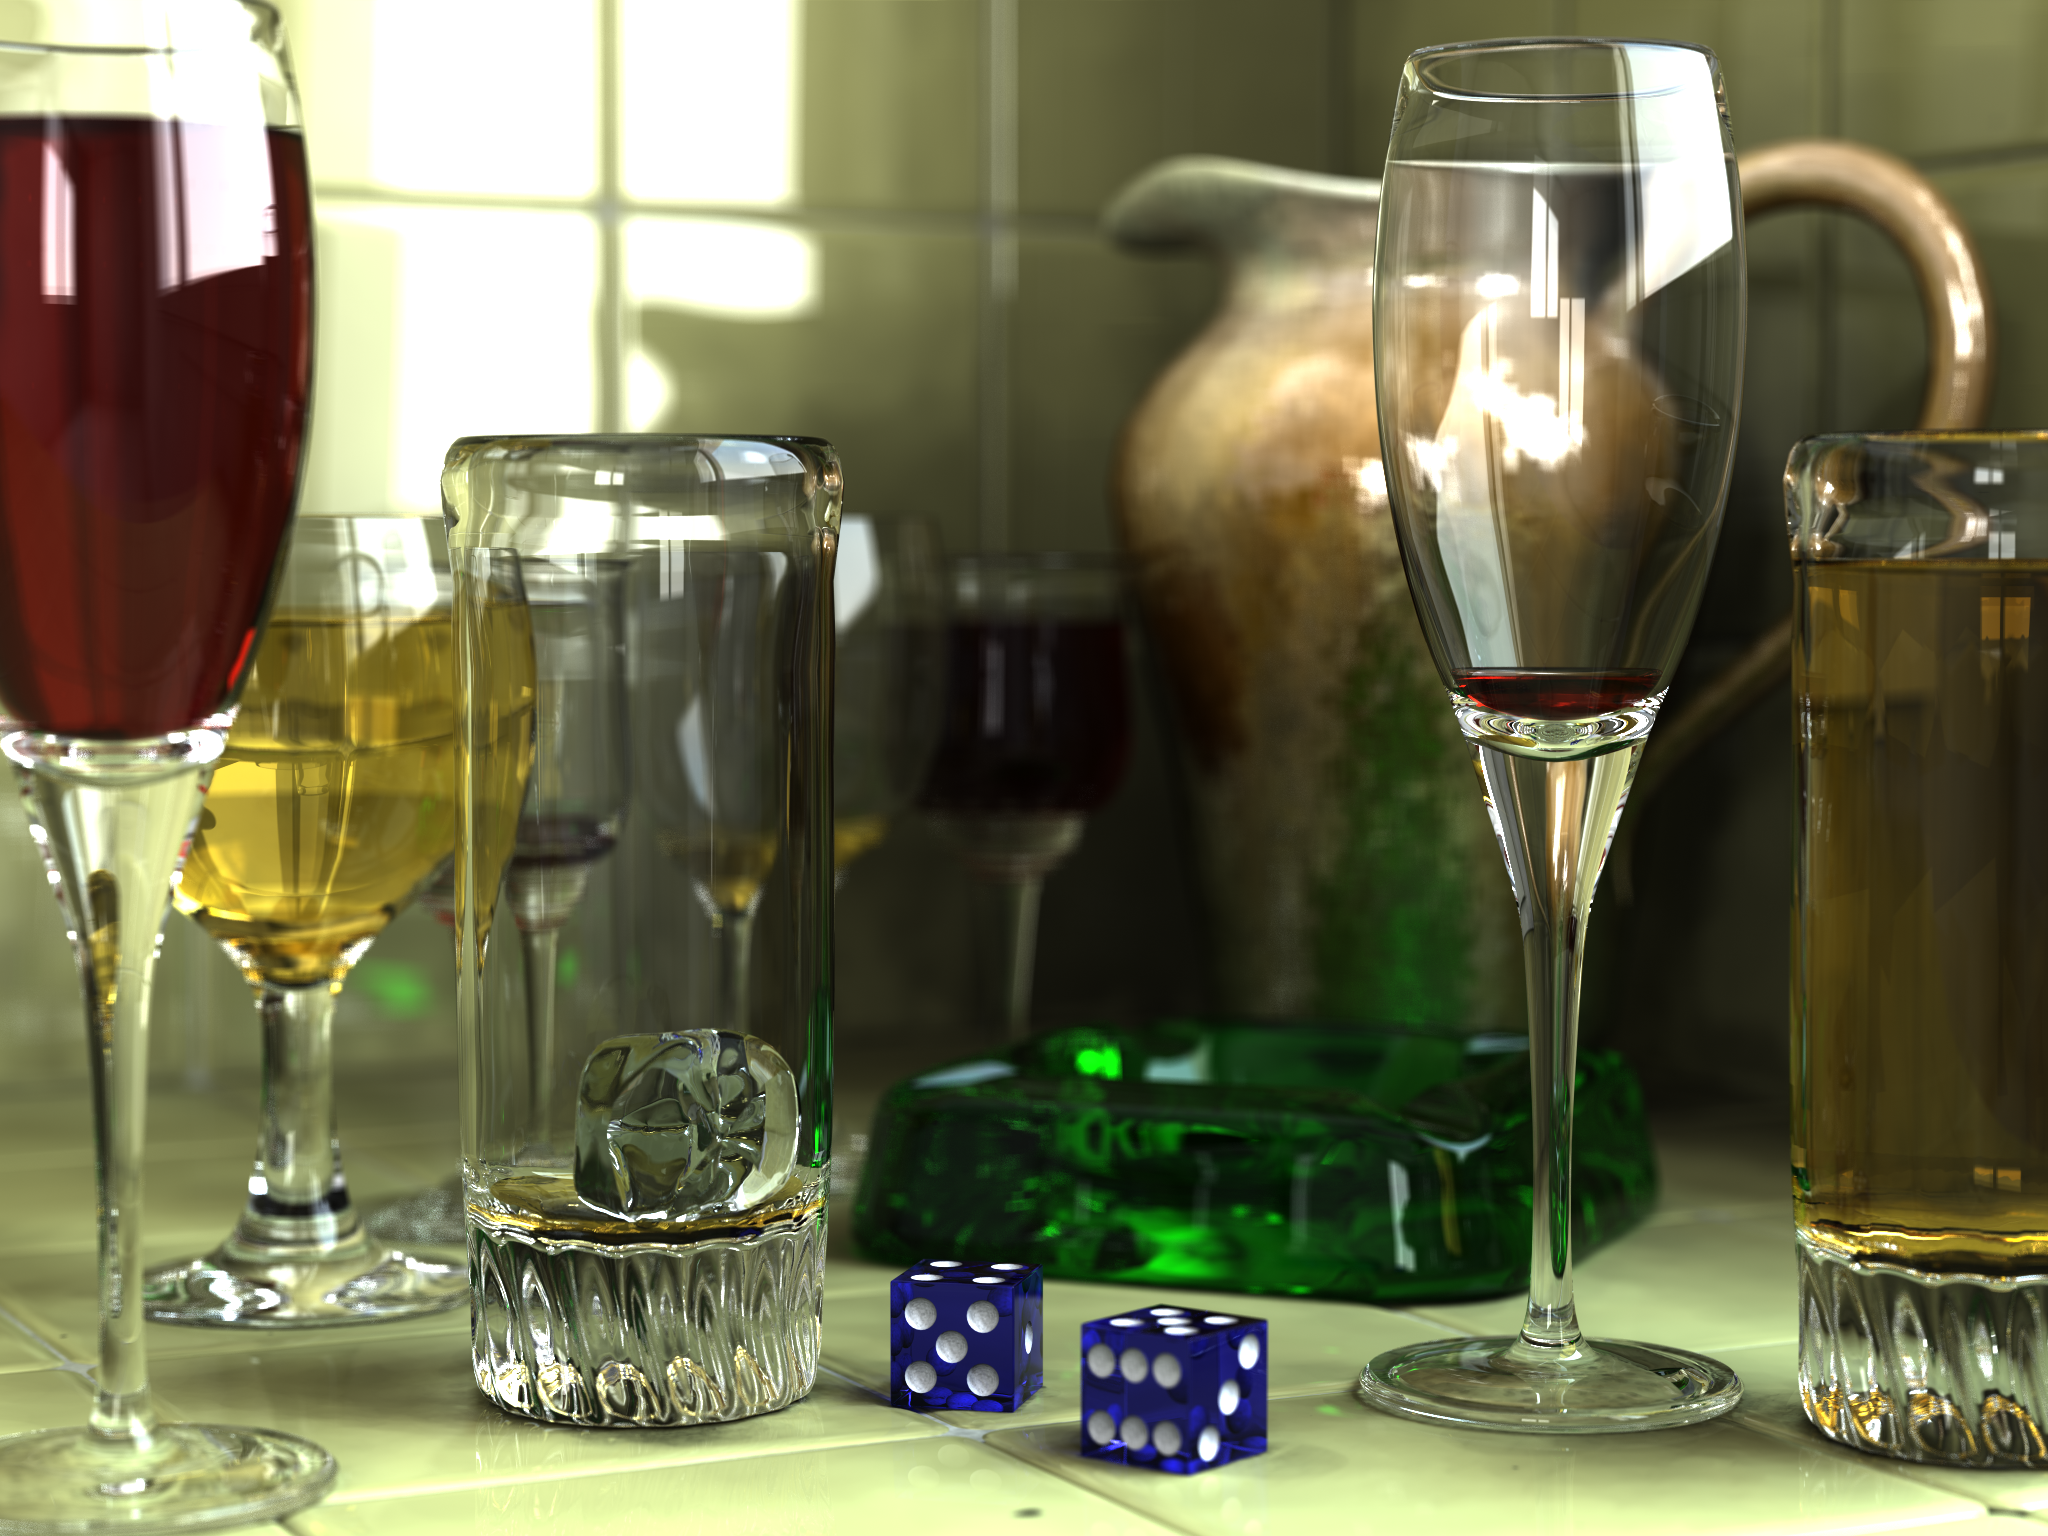
\includegraphics[width=0.8\textwidth]{resources/glasses_povray}
  \caption{POV-Ray render created by Gilles Tran \cite{povray2006render}}
  \label{fig:povray_render}
\end{figure}


Ray-tracing revolves around the idea of {\it rays}, a mathematical construct which can be defined by two vectors: an origin point, referred to as $\rayorg$ for some ray $R$, and a direction, referenced as $\raydir$.
These two vectors together represent a ray of infinite length that starts at the origin and projects along the direction.
An important addition to the concept of rays is a point along a ray -- this can be defined by using a third variable, $t$, to represent how far along the ray the point is located.
Therefore, Formula~\ref{equation:point_on_ray} can be used to get the coordinates of a point in three-dimensional space (assuming $\raydir$ is a unit vector).
This is called the {\it parametric~form} of a ray.
The mathematics behind ray-tracing are further explored in Section~\ref{sec:method}.

\begin{equation}
  \label{equation:point_on_ray}
  \vec{point} = \rayorg + t\raydir
\end{equation}

In ray-tracing, rays are used to simulate the path that light takes as it travels around the scene.
When a ray intersects with an object in the scene various interactions take place that simulate how light may travel under different conditions.
It is worth noting that a base assumption is made in ray-tracing when using straight rays as described here: light follows a straight line without changes.
This is only the case in reality when light travels through a vacuum with no gravitational bodies; thus, basic ray-tracing is not exactly photorealistic and does not model phenomena like atmospheric scattering.
Additional mathematics and systems must be used to bend, attenuate, or scatter a ray to accurately render transparent volumes -- this is called volumetric ray-tracing.
Volumetric ray-tracing will not be supported by the proposed \name, but would be a fascinating area of future work.

The basis for ray-tracing is the rendering equation, articulated by James Kajiya in 1986 \cite{kajiya1986rendering}.
The rendering equation models the outgoing light at some point given all incoming light, a bidirectional reflectance distribution function (BDRF), and a normal for the surface at the point modeled.
If solved for every point in the scene, the rendering equation could generate a completely photorealistic image -- this would, however, require massive amounts of computation.
This is because the rendering equation contains an integral over all incoming light which must be solved through numerical analysis.
Ray-tracing engines that do this are known as {\it path-tracers} and are the most photorealistic rendering engines invented.

\name\ will not use a path-tracer -- such algorithms are still many times too slow for most real-time rendering situations.
Instead, the rendering equation will be solved by sampling the incoming light with rays.
This is known as recursive ray-tracing, since it starts with a single ray that splits every time it encounters a surface.
The eventual goal of the recursive ray-tracing algorithm is to create a tree of rays for each {\it fragment} to render.
A fragment is either a pixel or some sub-pixel -- many systems will use four or more fragments per pixel to get better anti-aliasing and more accurate results.
Each ray contains some color that represents the color of the light in that ray.
When a ray hits an object, it is {\it scattered} by the {\it material} of the object, splitting and generating new rays.
These rays are biased towards directions that contain lots of incoming light -- such as towards a point light source.
The specific implementation of recursive ray-tracing that \name\ will use will only scatter into a set number of rays at each intersection point: one ray toward each light source, along with reflection and refraction rays towards the relevant directions.

The base of each generated tree is an {\it eye-ray} -- a ray with its origin at the fragment location on the camera plane.
The eye-ray's color is the color that will be rendered for that fragment.
As the eye-ray projects forward, away from the eye, it is tested for intersection with all objects in the scene.
When an intersection happens and the generated rays scattered, the eventual color values of the scattered rays are combined to produce the color of the original eye-ray.
This is done recursively to fully render the scene.


\subsection{Image Composition using Unicode Characters}
\label{sec:introduction:unicode}

Unicode is a character standard that allows anyone to reference many thousands of characters to compose text, no matter the environment around the text \cite{unicode}.
Some critical characters that \name\ will use are known as the {\it block characters} -- they are characters \texttt{U+2580} -- \texttt{U+259F}.
Relevant characters are shown in Figure~\ref{fig:unicode_characters}.
Contingent on the quality of the output using only block characters, additional sets could be used, such as triangles and lines.
The core of image composition using Unicode is an algorithm coloring the characters and the background -- \name\ will use this algorithm on every character of the output to both determine the character to display, and the foreground and background colors for that character.
The foreground colors the character itself, whereas the background provides a relief color.
This allows each {\it character~pixel} to represent a hard gradient.

\begin{figure}[htb]
  \centering
  \hspace{0.3em}
  \begin{subfigure}[htb]{0.4\textwidth}
    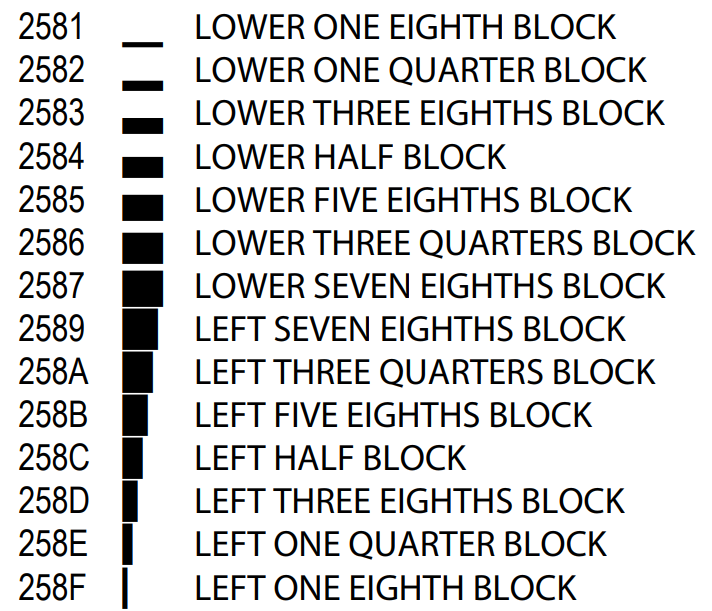
\includegraphics[width=\textwidth]{resources/block_elements}
    \caption{Block Elements}
    \label{fig:unicode_block_characters}
  \end{subfigure}
  \hfill
  \begin{subfigure}[htb]{0.51\textwidth}
    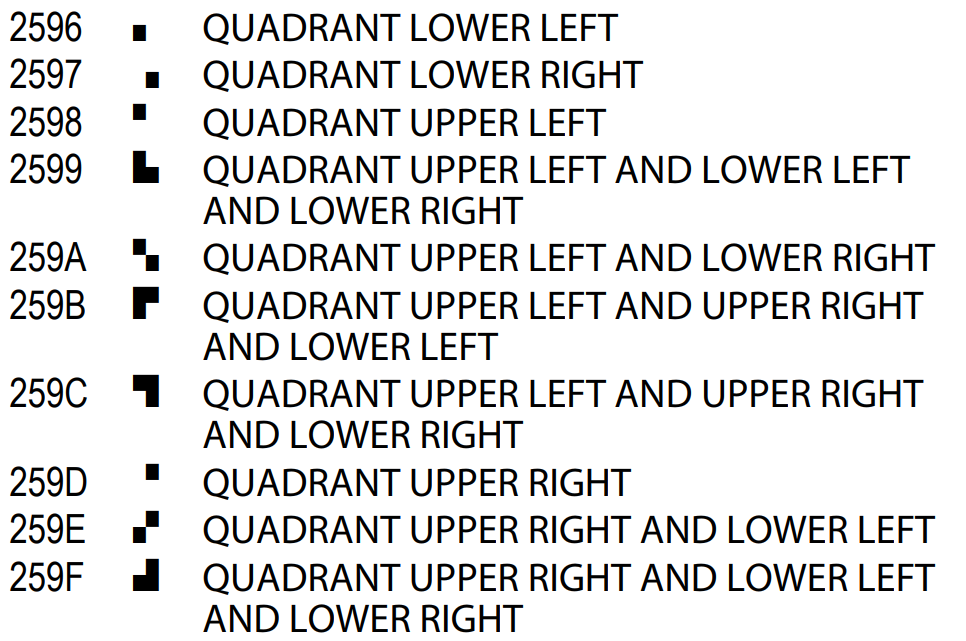
\includegraphics[width=\textwidth]{resources/quadrant_elements}
    \caption{Quadrant Elements}
    \label{fig:unicode_quadrant_characters}
  \end{subfigure}
  \caption{Subset of \texttt{U+2580} -- \texttt{U+259F}}
  \label{fig:unicode_characters}
\end{figure}

There are two image modes that will be available for use in \name.
The first is pure {\it pixel mode}, in which the Unicode ``half-block'' symbol (\texttt{U+2584}) is used.
Since mono-spaced character output (such as in a terminal) is twice as tall as it is wide, the half-block can split a single character into two pixels that are colored differently: the upper pixel with the background color of the character, and the lower with the character or foreground color of the pixel.
This would mean that a typical 85 by 30 character terminal would result in a screen space of 85 by 60 pixels.
This mode also dramatically reduces the number of ray-tracing computations needed, since only one ray per pixel is required.

The second image mode is considerably more complicated and slower, as it uses significantly more rays per character in order to determine what Unicode block character most fits the desired output.
On the other hand, it allows a much higher perceived resolution, since the characters used have smaller footprints of down to an eigth of a character in width or length.
The differences between these two modes are highlighted in Figure~\ref{fig:unicode_mode_comparison1} and~\ref{fig:unicode_mode_comparison2}.
It can be seen that the first image mode, {\it pixel mode}, shows a rather fuzzy definition of the main large sphere.
However, in the second image mode, {\it character mode}, the sphere and the reflections seen in it are much more defined.
The performance impact of both modes is another factor that must be assessed when making implementation decisions for \name.
More details on the algorithm for ray-to-character translation is available in Section~\ref{sec:method:ray_character_algorithm}.

\begin{figure}[htb]
  \centering
  \begin{subfigure}[htb]{0.49\textwidth}
    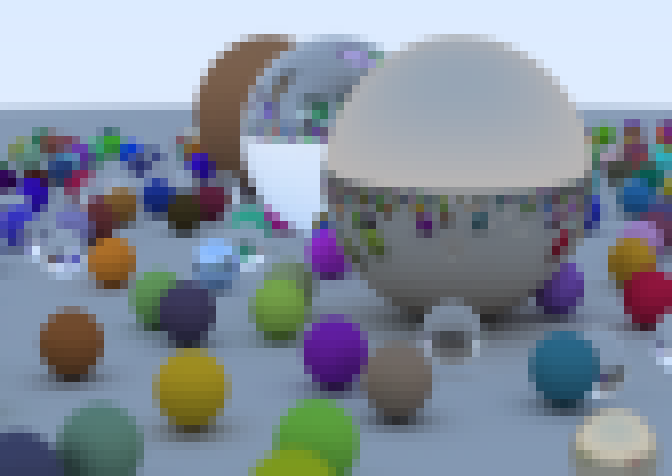
\includegraphics[width=\textwidth]{resources/many_spheres_square}
    \caption{Pixel Mode Image Output}
    \label{fig:unicode_mode_comparison1}
  \end{subfigure}
  \hfill
  \begin{subfigure}[htb]{0.49\textwidth}
    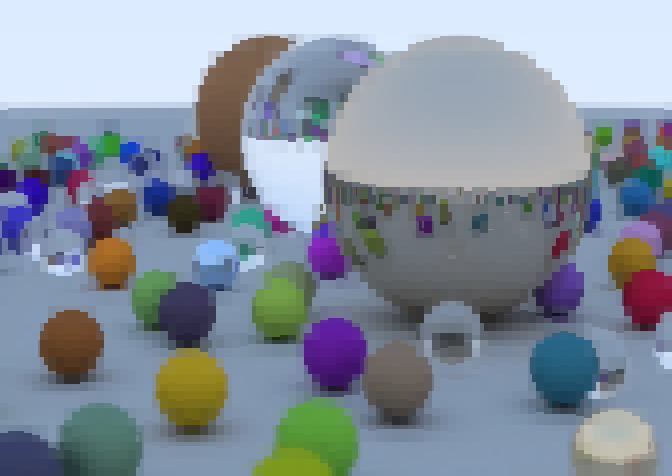
\includegraphics[width=\textwidth]{resources/many_spheres}
    \caption{Character Mode Image Output}
    \label{fig:unicode_mode_comparison2}
  \end{subfigure}
  \caption{Examples of Image Mode Output}
  \label{fig:unicode_mode_comparison}
\end{figure}

\subsection{Terminal Output using \texttt{ncurses}}
\label{sec:introduction:ncurses}

Once an image is generated, \name\ must somehow display that image in a terminal with no surrounding prompt or other formatting -- just a simple {\it character field}.
To do this, we will use \texttt{ncurses}, a C library that abstracts implementation details of the terminal to enable full-window 24-bit color character output.
Using \texttt{ncurses}, the terminal window will be divided into two ``panels'', a main panel for the actual image output -- updated 30 to 60 times per second -- and an info panel to render information such as frames per second and logging information.
With this dependency, \name\ can be used on all terminals that support \texttt{ncurses} -- generally, any XTerm-like terminal will work, as long as it supports a terminal information database: either \texttt{termcap} or \texttt{terminfo} will work.

A possible limitation to \texttt{ncurses} is keyboard input handling -- there is no mechanism to get events on an up or down movement of a key, as is possible in some other libraries.
Therefore, research will need to be done on possible alternatives for the input aspect of the engine.
This is not a priority, however, since it is not related to the rendering nature of \name and instead only helps with demonstrations of its capabilities.

\section{Related Work}
\label{sec:relatedwork}

% Summarize the previously published papers and books that are related to your proposed research.
% Whenever possible, you should compare and contrast your approach with the ones that have been discussed in the past.
% As you describe related papers, please make sure that you cite them properly~\cite{conrad-gecco-selection-study}.

In this section, we will discuss related research papers, detail how they inform \name's development, and show the improvements of \name\ over similar systems.
First, we will conduct a high-level discussion of the first ray-tracing paper all the way to modern-day optimizations and innovations.
Following that, we will discuss two Github projects, one of which has already been utilized to create the example figures such as Figure \ref{fig:unicode_mode_comparison}.


\littlesection{The First Ray-Tracer}

% To create an image, a ray-tracer first generates {\it eye-rays}, one for each pixel to render.
% These rays have their origin at the camera, and a direction which causes the ray to pass through the pixel to render.
% Each ray is then tested against all objects in the scene for intersection, and the intersection with the closest distance is chosen.
% This was the only thing the original ray-traced shading algorithm \cite{appel1968some} did, after which the amount of illuminance incident on the point the ray hit, along with some information available from other algorithms (such as if the surface faced a light), dictated the level of darkness of that pixel.
\todo{appel}

\littlesection{The Breakthrough}

\todo{whitted}

\littlesection{Formalization}

\todo{the rendering equation}

\littlesection{Accelerated Intersections}

\todo{acceleration structures}

\littlesection{Parallelization}

\todo{GPU ray-tracing}

\littlesection{TerminalImageViewer}

\todo{}

\littlesection{Gaming with \texttt{termloop}}

\todo{}

% rewrite above (use stuff on doc) and continue thread three

\section{Method of Approach}
\label{sec:method}

% Use technical diagrams, equations, algorithms, and paragraphs of text to describe the research that you intend to complete.
% See the \LaTeX\ source file for the proposal to learn how Figure~~\ref{intro-fig1} and Table~~\ref{intro-tab1} were included.
% Be sure to number all figures and tables and to explicitly refer to them in your text.

The methods, algorithms, and techniques used to implement \name\ are discussed here.
In Section~\ref{sec:method:algorithms} we detail most of the mathematics involved; core algorithms for the \texttt{ncurses} interface are also covered there.
Software tools and languages utilized to build \name\ are discussed in Section~\ref{sec:method:software}.
Finally, hardware interfaces, along with the current landscape of hardware availability, are covered in Section~\ref{sec:method:hardware}.
Additionally, discussion on parallelization is presented.

\subsection{Algorithms and Mathematics}
\label{sec:method:algorithms}
The mathematical basis for ray-tracing, which we describe in Section~\ref{sec:method:ray_surface_intersection_algorithms}, relies on an understanding of vector math.
These algorithms will be running millions of times per second in a highly parallelized environment; therefore, any small optimizations make huge differences in the end product.
We also cover details for the proposed algorithms for ray-to-character translations in Section~\ref{sec:method:ray_character_algorithm}.
All of the ray-tracing mathematics described here are synthesized from Peter Shirley's excellent {\it Ray Tracing in One Weekend} \cite{shirley2016ray} and the Morgan Kaufmann textbook {\it Physically Based Rendering: From Theory to Implementation} \cite{pharr2016physically}.

\subsubsection{Ray-Surface Intersection Algorithms}
\label{sec:method:ray_surface_intersection_algorithms}
Scenes that can be ray-traced must be a collection of surfaces that are mathematically intersectable with a ray.
Any surface that can be defined by $f(\vec{p}) = 0$, that is, $f(\vec{p})$ is $0$ when $\vec{p}$ is on the surface, is intersectable with a ray \cite{pharr2016physically}.
The point of intersection can be found by solving equation ~\ref{equation:ray_surface_intersection} for $t$ and then using formula ~\ref{equation:point_on_ray} to calculate the coordinates of that point on the ray.

\begin{equation}
  \label{equation:ray_surface_intersection}
  f(\rayorg + t\raydir) = 0
\end{equation}

In \name, the only surfaces that will be supported are spheres, triangles, and infinite planes, since their surface definition functions are mathematically simple.
If there is additional development time and resources available, other shapes such as quads, arbitrary polygons, and cubes may be considered; in fact, the algorithm discussed for triangle intersection testing is applicable to any convex polygon.
A sphere is the simplest object to calculate ray intersection with, and therefore will be the first implemented for \name.
In fact, during feasibility testing much of the math described in this section was implemented in the Go programming language.

\littlesection{Ray-Sphere Intersection}

The surface definition function of a sphere is function ~\ref{equation:sphere_surface}, with $S$ representing the sphere.
The intersection point between a ray and a sphere is given by solving equation ~\ref{equation:ray_sphere_intersection} for $t$ and then using formula ~\ref{equation:point_on_ray}.
Both of these equations are directly adapted from {\it Ray Tracing in One Weekend} \cite{shirley2016ray}.
Notice that equation ~\ref{equation:ray_sphere_intersection} is quadratic, and the number (and values) of the roots give us the $t$ we want to use.
The smallest positive root corresponds to the point on the ray which first intersects the sphere.
If there are no real roots, then the ray does not intersect the sphere.

\begin{equation}
  \label{equation:sphere_surface}
  f(\vec{p}) = (\vec{p} - \vec{S_{center}})^2 - {S_{radius}}^2
\end{equation}

\begin{equation}
  \label{equation:ray_sphere_intersection}
  (\raydir^2)t^2 + 2(\raydir \cdot (\rayorg - \vec{S_{center}}))t + (\rayorg - \vec{S_{center}})^2 - {S_{radius}}^2 = 0
\end{equation}

\littlesection{Ray-Plane Intersection}

For any two-dimensional object, the plane it lies in is the first shape tested for intersection; luckily, ray-plane intersection testing is fairly cheap and straight forward.
The surface definition function of a plane is function ~\ref{equation:plane_surface}, with $P$ representing the plane.
The plane's {\it offset} is a point on the plane, and the plane's {\it normal} is a vector perpendicular to the plane.
The intersection point between a ray and a plane is given by solving equation ~\ref{equation:ray_plane_intersection} for $t$ and then using formula ~\ref{equation:point_on_ray}.
These equations were derived from basic vector math, along with inspiration from {\it Physically Based Rendering} \cite{pharr2016physically}.

\begin{equation}
  \label{equation:plane_surface}
  f(\vec{p}) = (\vec{p} - \vec{P_{offset}}) \cdot \vec{P_{normal}}
\end{equation}

\begin{equation}
  \label{equation:ray_plane_intersection}
  (\vec{P_{normal}} \cdot \raydir)t + \vec{P_{normal}} \cdot (\rayorg - \vec{P_{offset}}) = 0
\end{equation}

%%%%%%%% {{ description of crossing-number algorithm (not used -- too complicated, likely not optimized) }}
% If this is used in the future should use P_{offset} as origin, not Q
% The method for testing intersection with triangles is a bit more complicated, but similar to tests for other polygons.
% First, intersection is tested with the plane the triangle lies in -- this results in a ray-plane intersection point $\vec{Q}$, or no intersection.
% Then, another test must be performed if there was an intersection to detect if $\vec{Q}$ is inside the triangle.
% Before we do this we must transform our coordinate system to 2D by projecting $\vec{Q}$ and the triangle's vertices  onto the plane.
% We can define our $\vec{X}$ and $\vec{Y}$ axes to be $\vec{X} = \vec{V_0} - \vec{V_1}$ and $\vec{Y} = \vec{P_{normal}} \times \vec{X}$; our origin we define to be $\vec{Q}$.
% Finally, we can use function~\ref{equation:3d_to_2d} to transform a three dimensional vector to a two-dimensional point on the plane.
%
% \begin{equation}
%   \label{equation:3d_to_2d}
%   f(\vec{w}) = [(\vec{w} - \vec{Q}) \cdot \vec{X},\ (\vec{w} - \vec{Q}) \cdot \vec{Y}]
% \end{equation}
%
% After converting our triangle vertices $\vec{V_0}, \vec{V_1}, \vec{V_2}$ to planar coordinates, we can test whether the triangle defined by them includes the origin $\vec{Q}$.
% We will do this using the ``crossing number'' method; first, create an arbitrary 2D ray with $\rayorg = [0, 0]$ and $\raydir = [0,\ 1]$.
% Then, we will use equation~\ref{equation:ray_line_intersection} -- the  ray-line intersection test -- to test each edge of the triangle to see if it intersects.
% If it does, we add one to the crossing number; then, after testing every edge of the triangle, if the crossing number is even $\vec{Q}$ is outside the triangle.
% Otherwise, $\vec{Q}$ is inside the triangle.

\littlesection{Ray-Triangle Intersection}

The method for testing intersection with triangles is a bit more complicated than the other tests we've covered so far.
The mathematics for this section are again derived from vector mathematics, however Jean-Colas Prunier's {\it Scratchapixel}, an excellent and accessible online resource for 3D rendering \cite{prunier2017triangle}, was an indispensable guide along the way.
First, intersection is tested with the plane the triangle lies in -- this results in a ray-plane intersection point $\vec{Q}$, or no intersection.
Then, if there was an intersection, another test must be performed to detect if $\vec{Q}$ is inside the triangle.
We do this using the ``inside-outside'' method (as suggested by {\it Scratchapixel}): test if $\vec{Q}$ is on the left side of each edge.
First, label each triangle vertex $\vec{V_i}$, with $i$ increasing in the counter-clockwise direction.
Thus we have three triangle vertices: $\vec{V_0}$, $\vec{V_1}$, and $\vec{V_2}$.
We can then use function~\ref{equation:left_edge_test}: if $f(i) > 0$ for each $i$, then $\vec{Q}$ is inside the triangle.
Otherwise, $\vec{Q}$ is outside the triangle.
Note that in function~\ref{equation:left_edge_test}, if $i = 3$, then $i = 0$ ($i$ ``wraps'' to only valid values).

\begin{equation}
  \label{equation:left_edge_test}
  f(i) = P_{normal} \cdot ((\vec{V_{i+1}} - \vec{V_i}) \times (\vec{Q} - \vec{V_i}))
\end{equation}

Function~\ref{equation:left_edge_test} can be complicated to visualize, so imagine this: we first form two vectors, both with $\rayorg = \vec{V_i}$.
One points along the triangle's edge, while the other points to $\vec{Q}$.
Both of these vectors will be in the plane of the triangle.
Thus, if we cross them, the vector produced will either be away from the plane in the same direction as $\vec{P_{normal}}$, or away from the plane in the opposite direction.
According to the right hand rule, if the crossed vector is in the same direction as $\vec{P_{normal}}$, then the vector pointing to $\vec{Q}$ is ``to the left'' of the vector pointing towards $\vec{V_{i+1}}$.
We can then get the dot product between $\vec{P_{normal}}$ and the crossed vector -- if it is positive then the crossed vector is in the same direction as the normal, and therefore $\vec{Q}$ is to the left of the edge.
One last addendum to this intersection test is the fact that it is very difficult to perform the counter-clockwise numbering of vertices -- therefore, we will simply expect vertices to be specified in counter-clockwise order.
This is similar to what many other 3D rendering programs assume.

%%%%%% Rendering Equation explanation
% \subsection{Rendering Equation}
% \label{sec:method:rendering_equation}
% Equation~\ref{equation:rendering} is a slightly simplified form of the rendering equation, removing properties dealing with the wavelength of light and time.
%
% \begin{equation}
%   \label{equation:rendering}
%   L_{out}(\vec{x}, \vec{w}) = L_{emit}(\vec{x}, \vec{w}) + \int_{\Omega} f_r(\vec{x}, \vec{v},\vec{w})f_i(\vec{x}, \vec{v})(-\vec{v} \cdot n) dv
% \end{equation}

\subsubsection{Ray-Character Translation Algorithm}
\label{sec:method:ray_character_algorithm}

To translate the color result of a ray-trace to an actual character pixel, we propose two algorithms.
These algorithms are inspired by the pixel-to-character translation algorithm used in TerminalImageViewer \cite{tivGithub} -- they are optimization attempts.
\name\ will start with the Quadrant Algorithm, and then research and testing will be conducted to see if it is possible to improve towards the Search Algorithm, without incurring too much performance cost.
If neither algorithm is able to produce an acceptable image quality, and running TerminalImageViewer's algorithm is possible in real-time (it will require $32$ rays per character pixel), then \name\ will use that algorithm instead of an optimized version.


\littlesection{Quadrant Algorithm}

The Quadrant Algorithm works with only four rays per character pixel.
These four rays will sample each of the four quadrants of the character, and give color values.
Once we have the four quadrant colors, we take the perceived brightness of each quadrant, using formula~\ref{equation:perceived_brightness}, where $C$ is the color in question \cite{finley2006hsp}.
Using the translated values we calculate an average brightness for the entire character.
Any quadrant which has a higher brightness is then considered ``on'', while any darker quadrants are ``off''.
Thus we determine which character from the set \texttt{U+2596} -- \texttt{U+259F}, which is a subset of the Unicode block characters that consist of all combinations of character quadrants, best represents the brightness gradient of the character pixel.
After this, we must determine the color of the foreground (``on'') and background (``off'') quadrants.
This is simply the average color value of the relevant rays -- with this computed we have the colors and character to use for the character pixel.

\begin{equation}
  \label{equation:perceived_brightness}
  {brightness} = \sqrt{0.299 {C_{red}}^2 + 0.587 {C_{green}}^2 + 0.114 {C_{blue}}^2}
\end{equation}

The Quadrant Algorithm's main problem is that it does not take into account color differences -- colors may be wildly different but have the same perceived brightness and if this is the case then the average color would not be an accurate representation of the character pixel.
The main way to combat this would be to determine the ``on''-ness of quadrants by a per-channel tonal range check, as TerminalImageViewer does.
Before making such optimizations, however, the algorithm must be tested with actual images.


\littlesection{Search Algorithm}

The Search Algorithm starts with a completely different premise than the Quadrant Algorithm -- it keeps track of what characters might be a good fit and, with each additional ray computed, narrows the list.
This algorithm must again use the criterion of ``on'' and ``off''-ness, to calculate what parts of the image should be foreground and which background -- with this comes the previous problem of possible color inaccuracy.
The Search Algorithm searches over characters from the set \texttt{U+2581} -- \texttt{U+258F}; these characters are blocks that range from one-eighth to seven-eighths in height, and the same in the width direction.
The character pixel is sampled with rays in a semi-randomized fashion -- first a vertical search of the pixel is conducted, attempting to find an edge between ``on'' and ``off''.
Then, a search across the horizontal of the pixel is conducted.
In both of these searches the non-relevant axis is randomized to ensure that a significant edge is not missed.
Figure~\ref{fig:ray_sample_run} shows an example of one such set of searches.

\begin{figure}[htb]
  \centering
  \begin{subfigure}[htb]{0.33\textwidth}
    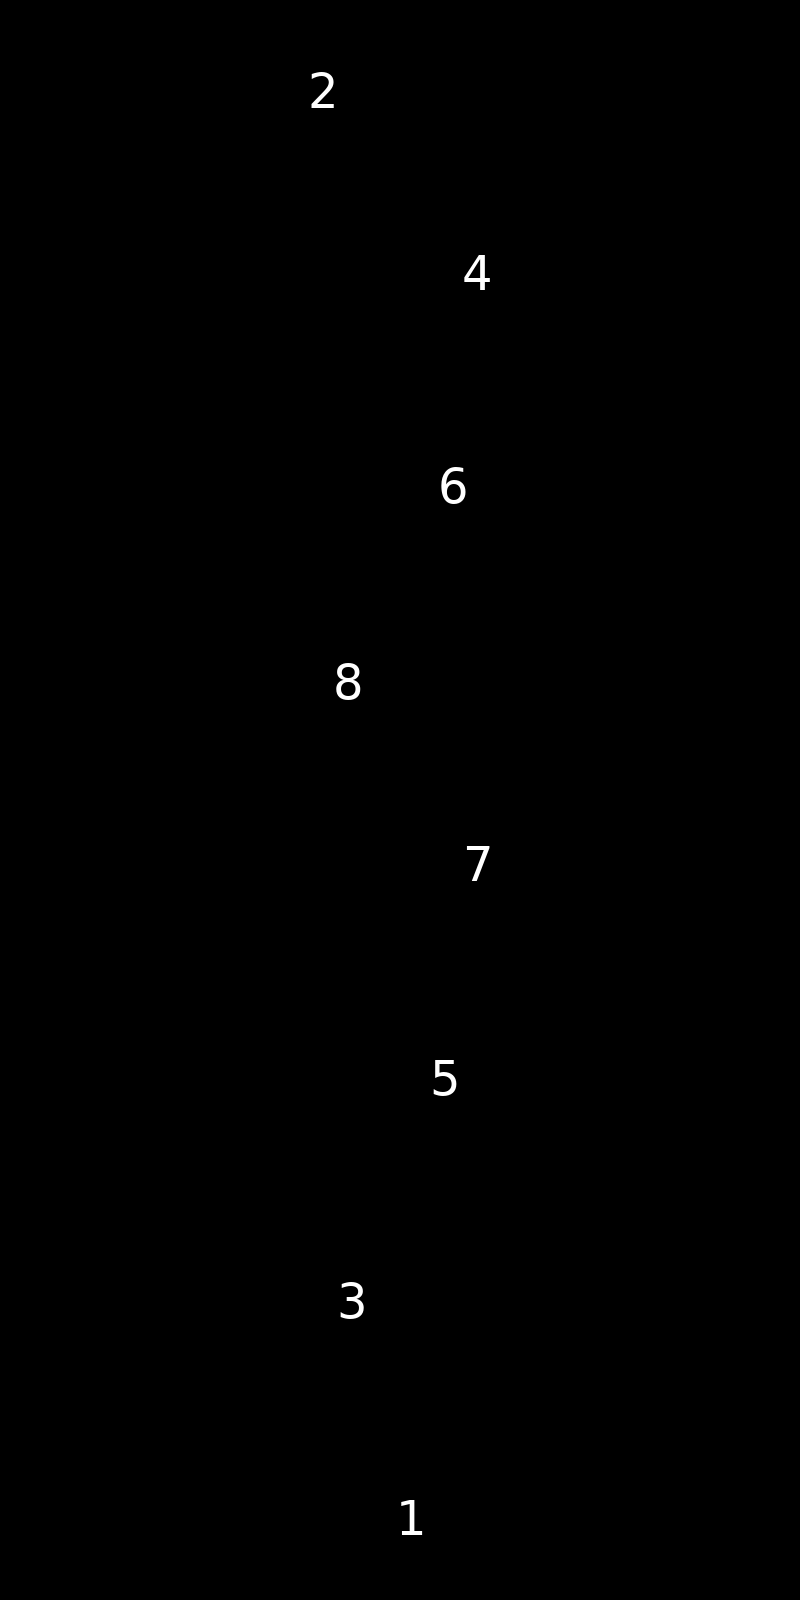
\includegraphics[width=\textwidth]{resources/height_search}
    \caption{Example randomized search over the character's vertical axis}
  \end{subfigure}
  \hspace{0.12\textwidth}
  \begin{subfigure}[htb]{0.33\textwidth}
    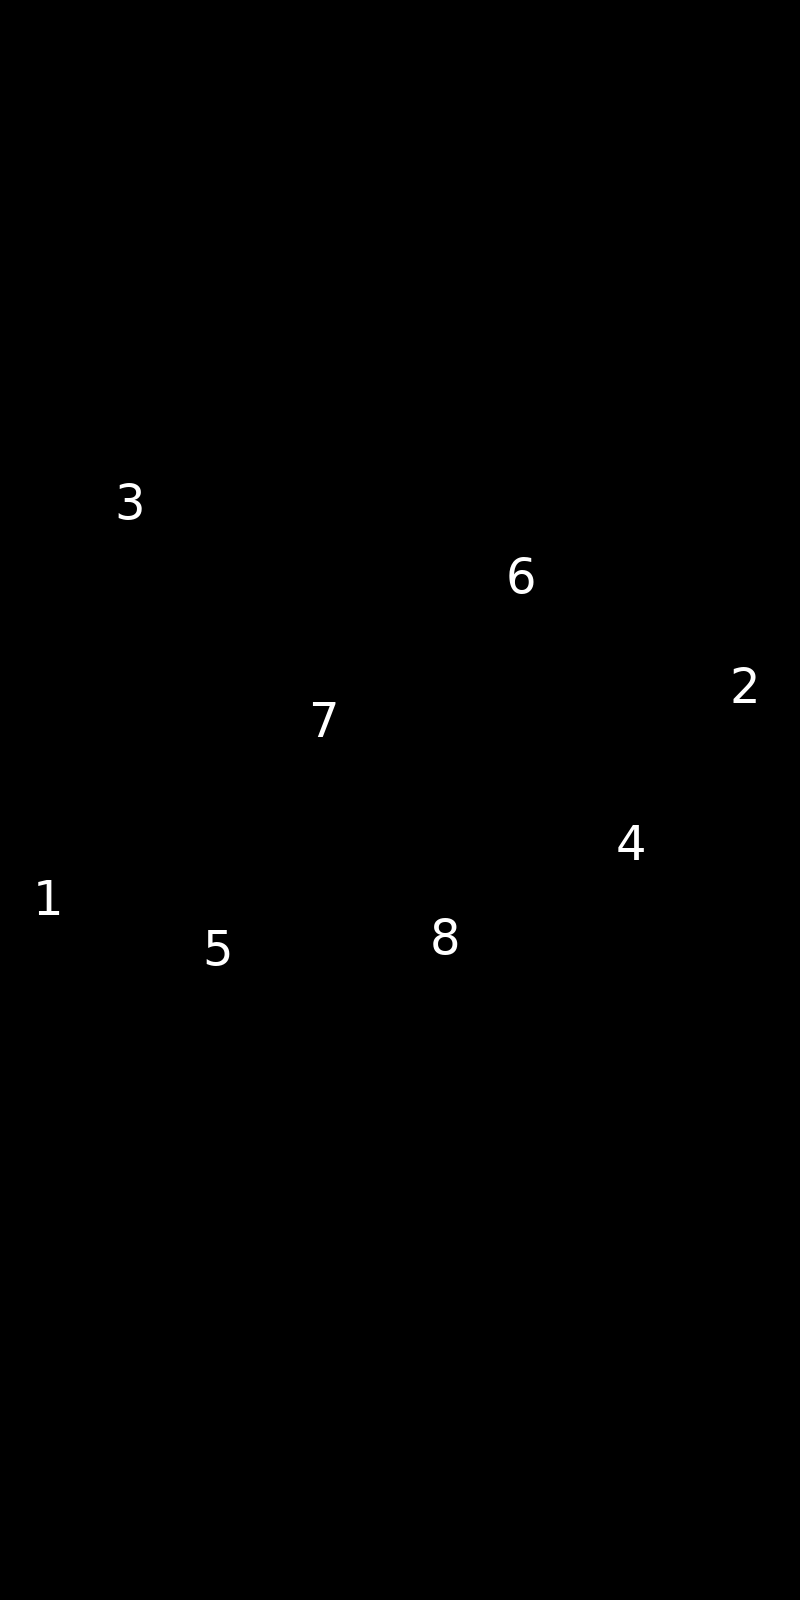
\includegraphics[width=\textwidth]{resources/width_search}
    \caption{Example randomized search over the character's horizontal axis}
  \end{subfigure}
  \caption{Example randomized searches -- numbers indicate processing order}
  \label{fig:ray_sample_run}
\end{figure}

Once the searches are complete, and an edge is found in both directions, the magnitude of the edges are tested.
The larger edge is then given priority, and the relevant character is selected -- for instance, if the vertical edge is given priority, and rays $1$, $3$, and $5$ (see Figure~\ref{fig:ray_sample_run}) are on, then the three-eighths tall block character (\texttt{U+2583}) will be selected for that character pixel.
This algorithm must also be tested with actual images, to judge the quality of the translation.
As with the Quadrant Algorithm, there are some possible optimizations for this algorithm -- most only apply to a sequential implementation; however, it would actually be faster to ray-trace all $16$ samples in parallel than to stop after every ray and check whether an edge has been found, as most optimizations would do.

\subsection{Software}
\label{sec:method:software}

\name's implementation will be hosted on Github, a public platform for projects using the Git version control system.
Travis CI \cite{travisci} -- a continuous integration system -- will be used for testing and environment management.
Documentation will be handled by \texttt{doxygen} \cite{van2008doxygen} -- all external facing functions, methods, and classes will have a minimum of a few sentences of documentation.
More details about the implementation tools are given in Section~\ref{sec:method:languages_and_libraries}.
Additionally, Section~\ref{sec:method:data_handling} discusses some implementation specific practices for handling data.

\subsubsection{Data Handling}
\label{sec:method:data_handling}

Data for use in scenes and materials will be stored in plain text.
This enables ease of use and human readability, as well as making scene editing extremely easy.
Data storage will likely use the YAML format, leveraging a C/C++ library or similar resource to ease the implementation burden.
The ideas described here are only informed guesses for how these entities should be represented; after the initial CPU ray-tracer implementation -- see Section~\ref{sec:schedule} -- this model may be improved.
Notably, one possible improvement is known as {\it instancing}, and involves allowing multiple copies of the same geometry to reference the same underlying data.

\littlesection{Materials}

Materials are not fully user-specifiable -- instead, they simply reference a type, such as lambertian or dielectric, and a texture.
Texture mapping is a complex topic that will require much more research, especially as implementation becomes a possibility.
For now, solid textures will be the only supported texture.
Some additional values such as metallic/reflectivity control specific aspects of the generated scattering function.
Materials also contain a user-set identification number to allow other objects to apply the material to themselves.

\littlesection{Objects}

Objects are composed of geometric primitives -- \name\ supports only spheres, infinite planes, and triangles.
Every object is recursively defined as a collection of sub-objects, or a primitive -- thus, a ``box'' object might contain four ``side'' objects when themselves contain two triangles.
Each sub-object is associated with an offset from its parent.
Thus, the data required for a geometry object definition is just an array of sub-objects and a position.
Every geometry object may have a material id -- if not specified, then the object's parent's material id is used instead.
This material id dictates what material is used to scatter rays when they intersect with the object.
Objects may also have an animation component -- a {\it movement path} -- identification number.
Similar to materials, movement paths are simply a collection of world locations and a length of time to take to traverse those locations.
In future versions of \name, these are likely to be removed in favor of total object control in the form of scripting integration.

\littlesection{Scene Description}

The scene description is a single file where all materials, objects, and movement paths in the scene are stored.
At the top level it contains three lists: one of materials, another of objects, and a third of movement paths.
One last special piece of data specific to the scene description is the camera description.
This specifies the technical details of the camera such as focal length and field of view, as well as mechanical details such as its position and speed.
The camera can also have a movement path defined, or optionally user control enabled.
User control enables the user to move the camera around in real-time, fully experiencing the ray-traced scene around them.


\subsubsection{Programming Languages and Tools}
\label{sec:method:languages_and_libraries}

With a large project such as \name, there are certain choices that must be made from a software development perspective.
These choices inform how the project is modified, built, and eventually executed.
In the case of \name, we chose to develop in the C++ language \cite{cpp14standard}, and use Gradle \cite{gradle} as the build system.
Hardware APIs are covered in Section~\ref{sec:method:hardware}.

\littlesection{C++}

The C++ language was chosen for three main reasons.
First, the language has a huge ecosystem of low-level tools, with interfaces to libraries such as OptiX, CUDA, FORTRAN-implemented mathematics like Blitz++, and much more.
This ensures that no matter the need, there is probably a library out there that will fill that need.
Secondly, C++ allows low-level C-like programming while keeping abstractions such as objects available.
Lastly, C++ is a reasonably fast language: with no virtual machine like Java or Kotlin, garbage collection is not a burden.
Decades of work have gone into compiler toolchains such as \texttt{g++} and \texttt{clang}, enabling optimizations that would not be possible for newer languages.

\name\ will attempt to keep most of its implementation to a C-compatible level, using classes and greater abstractions only as necessary.
This ensures that overhead will be minimal, as well as guaranteeing readability for the eventual open source release.
Advanced features of C++ such as templating will be avoided so as to keep the knowledge entry barrier low.
Finally, all code in \name's implementation will conform to the Google C++ style guide \cite{googleStyleGuide}.

\littlesection{Gradle}

Gradle is an opinionated build system that enables fully customizable tasks written in Java or Groovy.
It can be used to compile C++ code into a runnable executable using its Software Model.
This model allows the specification of specific executables and interdependent components, with sensible default source code locations.
Gradle efficiently manages long linking or dependency lists, without resorting to macro infested and variable filled makefiles; it also handles header inclusions seamlessly, without dealing with relative path issues.
Gradle can even automatically retrieve dependencies if they are published as a maven artifact.


\subsection{Hardware}
\label{sec:method:hardware}

There are a lot of unsolved technical issues that will be encountered as work continues for \name.
Much of this is related to the performance aspects of \name, since a high level of optimization is needed in order to obtain real-time results.
Only recently has ray-tracing even been able to achieve real-time levels of performance -- much of this progress is thanks to advances in GPU technology.
The largest innovator in this space, GPU chip design company NVIDIA, released its RTX series of GPUs that have hardware support for ray-tracing.
However, although fascinating, this proposal will not focus on RTX hardware, since its spread is slow due to the high early adoption cost.

The main technical research for hardware acceleration will be done on the OptiX API \cite{parker2010optix}, discussed in Section~\ref{sec:method:optix}.
The main goals of this research are to understand and use the technologies already available for non-real-time ray-tracing to do real-time work.
Hardware testing will be done on an Intel Core i7 4770k CPU and NVIDIA Geforce GTX 980Ti.

\subsubsection{GPU vs. CPU}
\label{sec:method:gpu_vs_cpu}

Although a CPU-only ray-tracer is completely possible, and will be the first step in embarking on the creation of \name, it is not likely to be performant enough for real-time graphics.
To reach this performance, the ray-tracer must take less than $\frac{1}{f\!\!ps}$ seconds to render a single image.
For $30$ frames per second, the minimum required for real-time fluid animation, \name\ must render an image every $33$ milliseconds.
Therefore leveraging either CUDA (a compute API for NVIDIA GPUs \cite{nvidia2011cuda}) directly, or utilizing OptiX will likely be required.

The main advantage to using a GPU instead of CPU is the massive parallelization possible -- GPUs often have hundreds to thousands of processor cores, whereas a standard CPU could have around eight.
Since ray-tracing is an inherently parallelizable algorithm, taking advantage of these extra cores provides massive boosts to performance, since many more rays are able to be simulated at once.
The problem is interfacing with the highly complex GPU architecture; often done through a shader program instead of some general purpose language.
Shader programs are bits of programmable code that is inserted between fixed operations such as vertex interpolation.
Since ray-tracing requires a completely different set of fixed operations, namely ray creation and intersection testing, it is not possible to use traditional methods.
Instead, a new interface must be used, such as the afore mentioned OptiX or CUDA.

\subsubsection{OptiX}
\label{sec:method:optix}

OptiX is an API interface developed for current generation NVIDIA GPUs that enables GPU-accelerated ray-object intersection calculations in a programmable graphics pipeline \cite{parker2010optix}.
OptiX allows user-defined single-ray {\it programs} to be compiled into a single program that runs on the GPU.
These programs are written in the PTX language.
Also available are acceleration structure implementations such as BVH.
Additionally, lightweight scene representation formats are defined and usable, although are not required for use of the main API.

Further practical research on the uses and implementation of OptiX is required, especially on the topic of C++ to PTX transpilation.
Additional research on the source code of OptiX itself may be useful as well, even if \name\ does not eventually use OptiX as an API.

\subsubsection{CUDA}
\label{sec:method:cuda}

Utilizing the massive parallel computation power of a GPU can be difficult -- in fact, before CUDA's release in 2007, there was no well defined way to do so programmatically.
CUDA is an API and computing platform that enables massively parallel computations.
A special extension of C++, known as CUDA C/C++, can be compiled with {\it nvcc}, a custom LLVM-based C/C++ compiler.
This extension enables library support for GPU accelerated multi-threading, physics, and linear algebra, along with many implementations of common data transformation algorithms.
A significant limitation, especially in the field of ray-tracing, is that performance is significantly effected for inherently divergent tasks -- tasks which do not consistently follow the same control flow -- such as traversing an acceleration structure.

\name\ may use CUDA C++ to perform ray-tracing intersection tests and dispatch ray simulations.
If OptiX, a more ray-tracing specific API, does not work out due to implementation issues or other reasons, CUDA is the fall-back resource.

\section{Evaluation}
\label{sec:evaluate}

% Explain what steps you will take to evaluate your proposed method.
% If you intend to conduct experiments, then you must clearly define your evaluation metrics.

Evaluation and testing of a graphics engine is a difficult proposition -- it often involves extremely subjective reasoning, especially as to the realism of an algorithm.
Given it's subjectiveness, some researchers use paired-comparison and rating-scale experiments \cite{kuang2007evaluating}.
These experiments generally ask observers to rate or compare the accuracy of some generated image.
\name\ will not be using these methods, as its purpose is not photorealistic graphics -- although adequate realism is expected -- but instead the unique pixelated style, as well as easy external use.

The original retro pixelated style has many critics and advocates, as can be seen in popular video game culture.
Therefore an observer-based test is likely to be heavily biased.
Instead of a comparison test by many participants, simple ``adequate realism'' tests will be conducted during development to detect bugs and focus implementation in the correct direction.
Descriptions of these tests, along with details on code testing, are available in Section~\ref{sec:evaluate:testing}.


\subsection{Portable Pixmap Output Mode}
\label{sec:evaluate:ppm_mode}

The first step in evaluating and testing a ray-tracer is to get the output in an versatile format -- for \name, a debug mode called {\it \texttt{ppm} mode} will generate image files in portable pixmap format.
This mode will be a different interface in addition to the \texttt{ncurses} character output modes, allowing much higher resolution output for testing.
It is unlikely that this will be real-time capable, but render times for \texttt{ppm} images with millions of fragments will serve as good benchmarks for algorithm optimizations.
The image format \texttt{ppm} was chosen for it's human readability along with ease of use for development -- it has both ASCII and binary forms, with the ASCII being more useful in our case.
The format is extremely simple; a \texttt{ppm} file is shown in Figure~\ref{fig:ppm_code}, with Figure~\ref{fig:ppm_image} being its output.

\begin{figure}[htb]
  \begin{subfigure}[htb]{0.5\textwidth}
    \small
    \vspace{2.6em}
    \begin{verbatim}
      P3 # header
      3 2 # width x height
      255 # max color value
      # image data -- RGB triplets
      # (extra whitespace is ignored)
      255   0   0     0 255   0
        0   0 255   255 255   0
      255 255 255     0   0   0
    \end{verbatim}
    \caption{\texttt{ppm} file contents}
    \label{fig:ppm_code}
  \end{subfigure}
  \begin{subfigure}[htb]{0.5\textwidth}
    
\includegraphics[width=\textwidth]{resources/ppm_example}
    \caption{\texttt{ppm} image}
    \label{fig:ppm_image}
  \end{subfigure}
  \caption{Portable pixmap format example}
\end{figure}

Using this \texttt{ppm} image output mode will enable graphical quality comparisons, testing, and bug-fixing.
It will also provide output and results data for output-based regression testing, to ensure that any changes are purposeful.
Lastly, \texttt{ppm} mode will be used to test the fidelity of \name's ray-to-character translation algorithm against other available algorithms in programs such as TerminalImageViewer by providing a single, identical input image for translation.
Both algorithms will be run, and the resulting character field evaluated for differences.


\subsection{Demonstration Scenes}
\label{sec:evaluate:demo_scenes}

In addition to \texttt{ppm} mode, demonstration scenes will also be built to enable real-time testing of the ray-tracing algorithm and \name's associated systems.
These scenes will provide data for ``adequate realism'' tests as well as provide demonstrations of \name's capabilities.
The final project will include at least the following scenes, but may be more extensive.

\begin{itemize}
  \setlength\itemsep{-0.25em}
  \item Whitted's Sphere
  \item Cornell's Box
  \item Shadow Demo
  \item Moving Object
  \item Environment Exploration
\end{itemize}

The first two scenes are famous ray-tracing reference scenes and will be used to benchmark the performance of \name\ against other ray-tracing engines, such as OctaneRender or Blender.
With the addition of the {\texttt{ppm}} image mode, output images will be visually compared to detect errors in visual effects such as specular reflections.
The other three scenes are demonstrations designed to showcase certain aspects of \name.
The Shadow Demo scene is a simple scene similar to NVIDIA's RTX shadow demo, seen in Figure~\ref{fig:nvidia_shadows}.
It will demonstrate soft shadows and show the limitations of \name's ray-tracer, since, at least at the moment, only point lights will be supported.
When this scene is implemented, and if there is time in the development schedule, area lights may be implemented through multiple random sampling.
This simple addition to recursive ray-tracing simply adds more shadow rays to each scatter, randomly spread between any area lights in the scene.

\begin{figure}[htb]
  \centering
  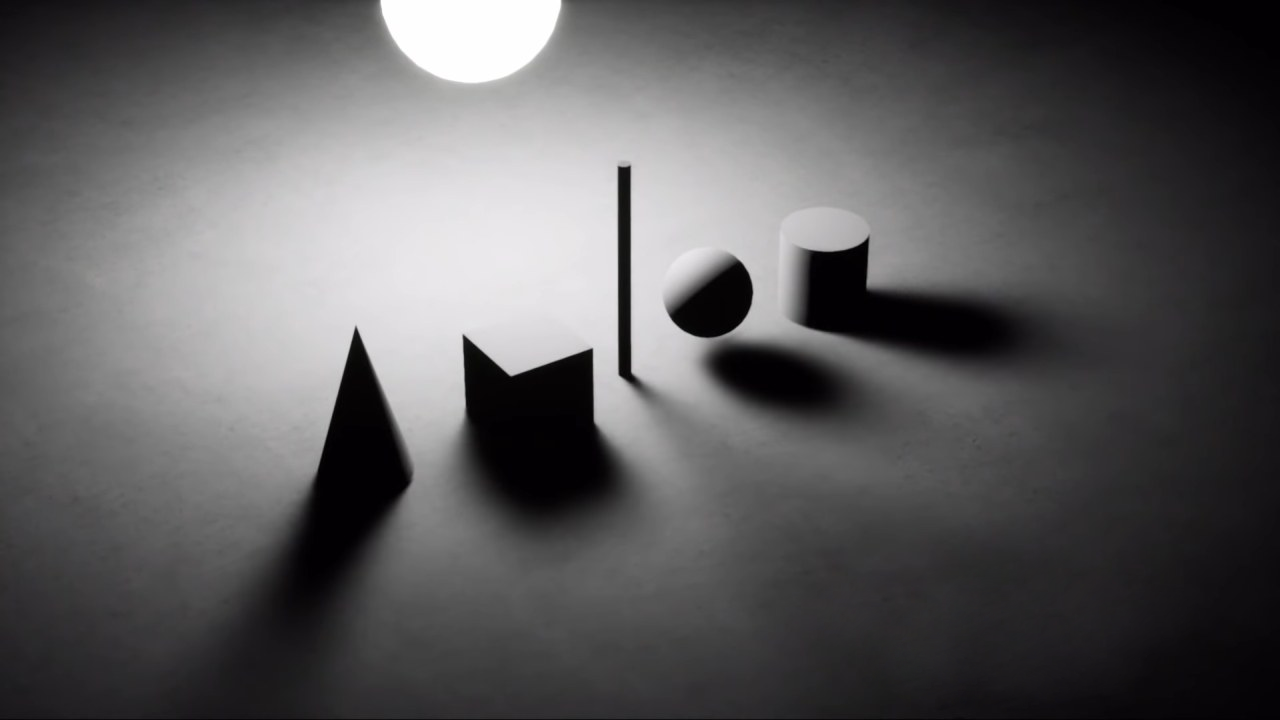
\includegraphics[width=\textwidth]{resources/nvidia_shadows}
  \caption{NVIDIA Shadow Scene -- shown at CES 2018, NVIDIA Keynote}
  \label{fig:nvidia_shadows}
\end{figure}

The Moving Object scene will be modeled after a typical Cornell Box, however the main point of the scene will be object and light source movement -- animated in real time.
This will stress the ray-tracer and demonstrate the real-time shadows, lighting, and rendering to the fullest extent.
Finally, the Environment Exploration scene is a somewhat nebulous idea -- it is a scene where the user will be able to ``explore'' and move the camera around to experience a wider area.
Currently envisioned as a set of complex models of a street corner or otherwise realistic location, it will be the stress test for \name.
As many thousands of objects and possibly millions of rays are computed per second, this scene will ensure that the ray-tracing algorithm is well-designed and optimized, and if an acceleration structure is implemented, it performs well.

Along with the scene demonstrations there will also be material demonstrations -- although simple in nature, they will show off the different implementations of lambertian, dielectric, and metal materials, along with other possible effects such as glass, tessellation, and ray-traced bump mapping.
Many of these effects are contingent upon available development time; however, at least the lambertian and metal demonstrations will be available in the final project.


\subsection{Testing}
\label{sec:evaluate:testing}

Testing will focus on reference image comparison, specifically with reference images generated by {\it Cycles}, the rendering engine used by the Blender modeling tool \cite{blender}.
These reference images will be compared with the same scene rendered with \name.
Visual effects such as reflections, specular highlights, transparency, shadows, and ambient occlusion will be examined in both images to determine if there is any loss of quality with \name's ray-tracing algorithm.
Some loss of quality is acceptable; however, anything that could be noticed by a viewer as appearing unrealistic or otherwise not making physical sense violates the ``adequate realism'' criterion.
An example of such a violation might be ``fireflys'' -- pixel abnormalities that are often colored black or white instead of the correct color -- caused by numerical errors.
Additional violations may occur in object seams or other areas where geometry is not fully defined -- these situations should be fixed if and when they occur.

The reference images and \name\ output will also be mathematically compared by highlighting portions of the images that are not pixel-perfect copies (often referred to as ``diffing'').
This is likely to have many false positive bug identifications, as small variations can easily happen, but could point out possible inaccuracies that do not appear physically incorrect but may still be a bug or unintended side effect.
Additional testing will focus on render times -- the time it takes a rendering engine to complete an image -- specifically comparing \name\ to OctaneRender \cite{octane} and its real-time ray-tracing algorithm.
This will involve creating identical scenes and then gathering and comparing performance data for both engines.
In most cases, since \name\ will be implementing only a subset of the effects OctaneRender uses, it should be faster.
As a counter-point, however, OctaneRender is highly optimized and thus may have the edge in raw performance for complex scenes.

Code testing will use the {\it Google C++ Testing Framework} for unit testing \cite{googletest}.
Code coverage should cover all mathematics routines at minimum, and greater than $90\%$ algorithm coverage is the goal.
CUDA or OptiX code testing will be done with a mix of CPU-side Google Test code and custom test handlers for GPU testing.
Unit testing for the \texttt{ncurses} interface should also be greater than $90\%$ if possible, however additional research into this area will be required, as mocking the terminal may prove to be more work than it is worth.
Lastly, test integration with Travis CI is also a goal.
Travis CI environment tests will also be used for different terminal types if additional research determines this is possible.

\section{Research Schedule}
\label{sec:schedule}

% Identify the main phases and tasks of your research project and set deadlines
% for when you will be able to complete each of these items.

Table~\ref{worktable} proposes a schedule for the implementation and research work needed to complete \name.
First, a CPU implementation of the recursive ray-tracing algorithm will be developed, at first tested in \texttt{ppm} output mode.
Then, as the ray-tracing code grows to a testable state, the \texttt{ncurses} interface will be developed.
This involves implementing the ray-to-character translation algorithm, as well as standardizing an interface with which another render engine (specifically the future GPU ray-tracer) can interface with the displayed terminal image.

\begin{table}[htb]
  \vspace*{0.6em}
  \centering
  \begin{tabular}{|c||c|c|}
    \hline
    \textbf{Task} & \textbf{Begin Date} & \textbf{End Date} \\\hline\hline
    Proposal defense preparation & Early Nov. & Mid Nov. \\\hline
    CPU implementation & Late Nov. & Early Jan. \\\hline
    \texttt{ncurses} interface implementation & Mid Dec. & Late Jan. \\\hline
    Thesis introduction/related works & Late Nov. & Mid Dec. \\\hline
    OptiX/CUDA research & Mid Dec. & Early Jan. \\\hline
    GPU implementation & Early Jan. & Early Feb. \\\hline
    Scene/material creation & Mid Dec. & Late Mar. \\\hline
    Thesis chapter writing & Early Feb. & Early Apr. \\\hline
    Graphical testing/comparison & Early Mar. & Mid Mar. \\\hline
    Thesis defense preparation & Early Apr. & Mid Apr. \\\hline
  \end{tabular}
  \caption{Proposed work schedule}
  \label{worktable}
\end{table}

Once both the CPU ray-tracer and \texttt{ncurses} implementations are nearing completion, research will begin on OptiX/CUDA integration.
The design and architecture of the GPU ray-tracer will take the lessons learned in the implementation of the CPU ray-tracer and use them to improve organization and understandability.
Additionally, the GPU ray-tracer will be highly parallelized, and so extra care must be taken to avoid the problems that are involved with parallelization.
Before the design phase for the GPU ray-tracer starts, thesis writing will commence in earnest.
The first stages of writing will document the challenges and lessons learned from completing the CPU ray-tracer, including performance testing and evaluation; these will eventually end up in the Methods of Approach section of the thesis document.
Additional research and writing for the Introduction and Related Works sections will also begin at this time.

Finally, implementation of \name's actual GPU ray-tracing engine will begin in early January.
From this point onward, implementation and demonstration will be the primary goals.
By late February, final demonstration scene creation should be wrapping up and material demonstrations should be well on their way to completion.
The tempo of thesis chapter writing picks up early March, with discussions of the various new GPU-based techniques used for the GPU ray-tracer as the primary focus.
Finally, end result testing and graphical comparisons will be conducted and documented, along with preparation for the thesis defense.

\section{Conclusion}
\label{sec:conclusion}

% Provide a summary of your proposed research and suggest the impact that it may have on the discipline of computer science.
% If possible, you may also suggest some areas for future research.

\name\ is a complex system, the implementation and design of which will not be fully known until initial testing and research is completed in the form of the CPU ray-tracer.
The proposed system will support real-time 3D scene viewing through a terminal emulator such as Konsole.
This will made possible by leveraging one of the hardware interfaces discussed in Section~\ref{sec:method:hardware} to compute ray-surface intersections in a highly parallelized manner on a GPU.
Ray-to-character translation algorithms are also needed to transform the rendered image into Unicode characters.
These algorithms, along with the \texttt{ncurses} library, enable \name's treatment of a terminal as an image canvas.

The development of \name\ will proceed at first in an experimental stage, while the abstractions and foundation for ray-tracing in general are created.
The end result of this stage is a working CPU ray-tracer, which may or may not be capable of real-time rendering.
The second and final stage involves rewriting the ray-tracer to utilize GPU compute power, enabling faster render times and real-time performance.
The lessons learned from the experimental stage are crucial for a good design and implementation at this point.
The end result of this stage is ultimate goal of \name\ -- a fully real-time capable ray-tracing engine, rendering 30 Unicode character images per second to a terminal window.

After the initial development period discussed in Section~\ref{sec:schedule}, all contributions to \name\ development will be welcome.
In the pursuit of maintaining good open-source readability and ease of development, documentation will be a priority throughout the initial implementation process.
Additionally, tight integration with Github and Travis CI will ensure the integrity of public contributions.
We hope that future projects will find \name\ inspiring and useful, whether as an engine or as a jumping-off point for real-time ray-tracing and terminal-based games.


\bibliographystyle{plain}
\bibliography{senior_thesis_proposal}
\end{document}
